%****************************************************************
% Chapter X
%****************************************************************
\chapter{Performance}
\label{chapter-performance}

%****************************************************************
What is great about the Android runtime is that most of the stress of memory reclamation is done for developers. The system will track what developers are doing and when it sees that an object is not needed anymore, it will free it on their behalf. However, this does not exclude performance problems from happening here. When the amount of memory have allocated reaches an upper limit, a Garbage Collection (GC) event will be kicked off to free any resources that might not be needed any longer, freeing up space for future allocations. 

Anytime the frame drips about the $16$ms barrier, and the users are going to start to notice. Therefore, any code that forces allocated memory to spike above this threshold can cause problems. For instance, memory can become tighter, if the developer is allocating and freeing a large number of objects in a short period of time, the temporary objects again kicking off GC event. 

\begin{figure}[H]
\caption{16ms Per Frame}
\label{fig:16ms-per-frame}
\centering
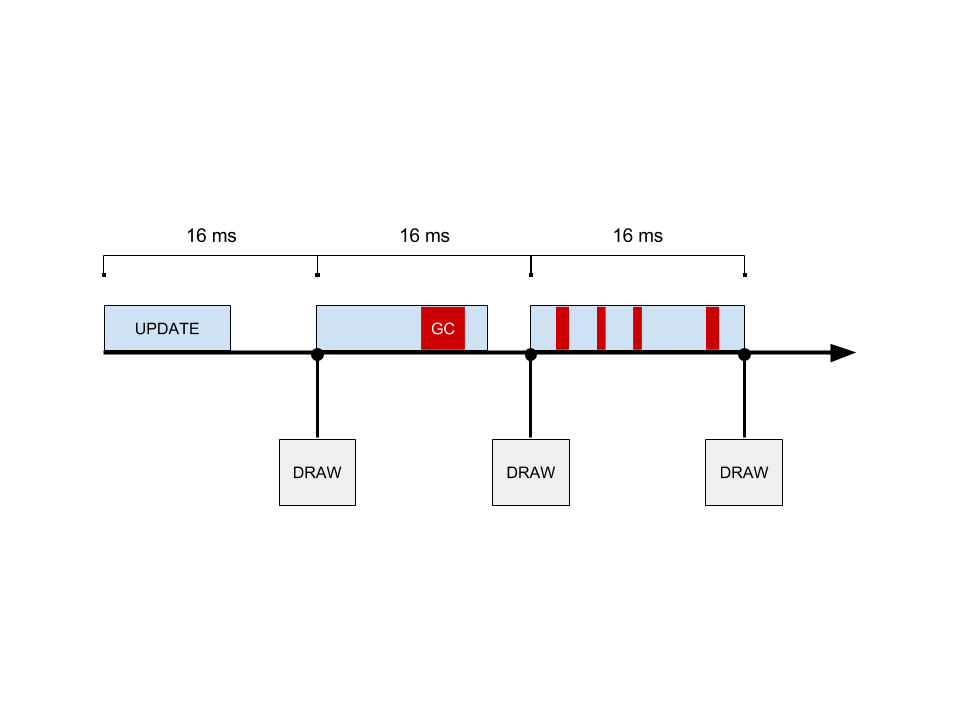
\includegraphics[width=\textwidth, keepaspectratio]{Figures/16ms-per-frame.png}
\decoRule
\end{figure}

Therefore, a performance testing is important for avoiding nasty GC events. Each GC event that developer can avoid, the application has more time per frame to do interesting things. In order to find out where in the code objects are being created but not released, created and not used, or created new when the developer could have been reusing them from existing objects. Android Studio provides a series of performance testing tools, such as Memory Monitor, Allocation Tracker, Heap Viewer, and the Systrace (it is an Android system trace tool helps developers analyze how the execution of the application fits into the many running systems on an Android device \cite{google.systrace.2016}). According to the runtime, the performance analysis is divided into two parts: acyclic process and cyclic process (performance data came from Android phone $Nexus\;6P$ \footcite{CPU: 2.0GHz octa-core, 64-bit ARM Cortex-A57 & ARM Cortex-A53, 8 cores; GPU: Adreno 430}).

%****************************************************************
\section{Initialization}

%****************************************************************
In order to avoid UI being block, all of acyclic process in the application are handled in the new threads. In this section, I present the performance of geometric vertices' generation for \code{Placemark} (Icosphere) and \code{Earth} (UV Sphere) which only executes one time (or not) when needed. The geometric data from Icosphere generation will be cached once it has been created. This is useful to avoid duplicate creations for same geometric vertices. In the \code{Placemark} description URL analysis, the same cache solution for image and text.

%****************************************************************
\subsection{Icosphere Generator}

%****************************************************************
Based on the varying roundness of the Icosphere, it could evolve into spheres have different vertex count. In general, level $3$ Icosphere is enough for illustrating a sphere, and in the application the \code{Placemark} is created on level $1$ Icosphere. As we can see from Chart \ref{fig:icosphere-performance} and Table \ref{tab:icosphere-level}, even for a particular reason that requires a level $5$ Icosphere, less than $300$ms is acceptable as an one time execution.

\begin{figure}[H]
	\caption{Icosphere performance}
	\label{fig:icosphere-performance}
	\centering
	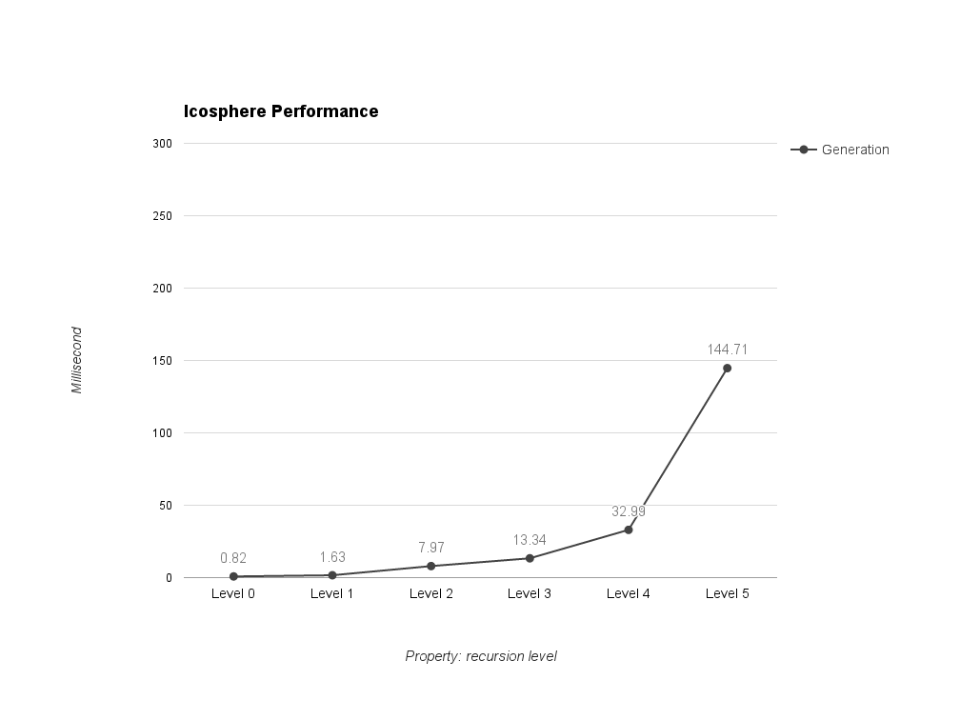
\includegraphics[width=\textwidth, keepaspectratio]{Figures/icosphere-performance.png}
	\decoRule
\end{figure}

\begin{table}[H]
\caption{Icosphere Level}
\label{tab:icosphere-level}
\centering
\begin{tabular}{l l l l}
	\toprule
	\tabhead{Recursion Level} & \tabhead{Vertex Count} & \tabhead{Mean Value (ms)} & \tabhead{Stand Deviation (ms)}\\
	\midrule
	0 & 12 & 0.049 & 0.014 \\
	1 & 42 & 0.257 & 0.490 \\
	2 & 162 & 0.722 & 0.250 \\
	3 & 642 & 3.296 & 0.707 \\
	4 & 2562 & 19.988 & 3.050 \\
	5 & 10242 & 148.927 & 18.422 \\
	\bottomrule
\end{tabular}
\end{table}

%****************************************************************
\subsection{UV Sphere Generator}

%****************************************************************
The roundness of a UV Sphere depends on the partition level on both horizontal (ring) and vertical (segment) which denotes the axes of the 2D texture. The Earth is casually implemented as a $180 / 180$ UV Sphere in the application.

\begin{figure}[H]
	\caption{UV Sphere performance}
	\label{fig:uv-sphere-performance}
	\centering
	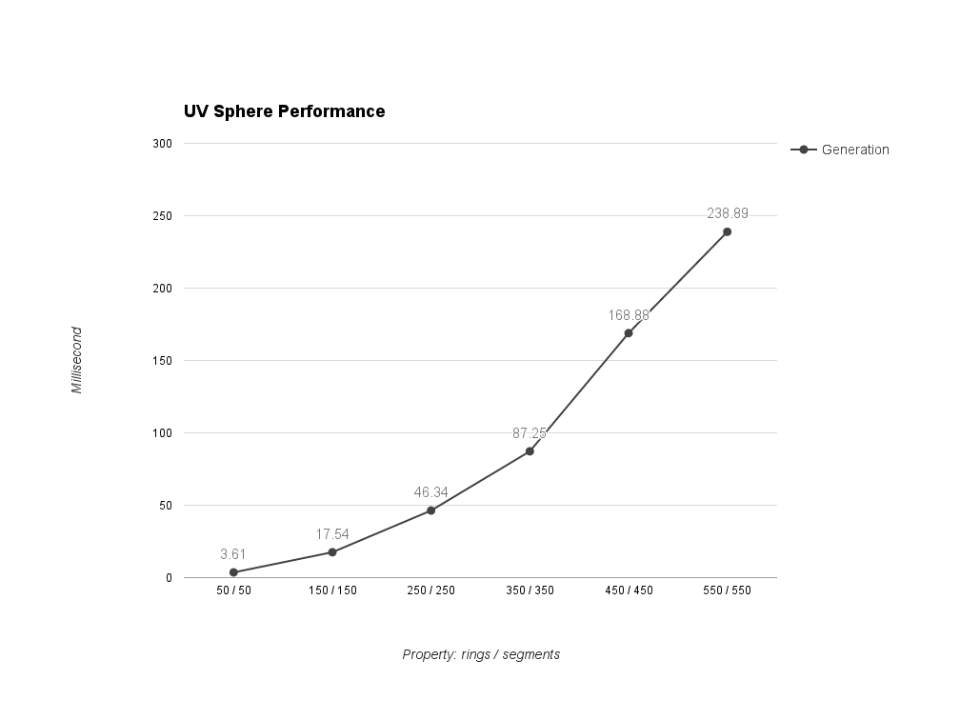
\includegraphics[width=\textwidth, keepaspectratio]{Figures/uv-sphere-performance.png}
	\decoRule
\end{figure}

%****************************************************************
\subsection{Geographic Data Initialization}

%****************************************************************
Figure \ref{fig:geographic-data-performance} is the performance of initializing geographic data, including parsing KML files, transformation coordinate system from LLA to ECEF for each \code{Placemark}, etc.

\begin{figure}[H]
	\caption{Geographic Data Performance}
	\label{fig:geographic-data-performance}
	\centering
	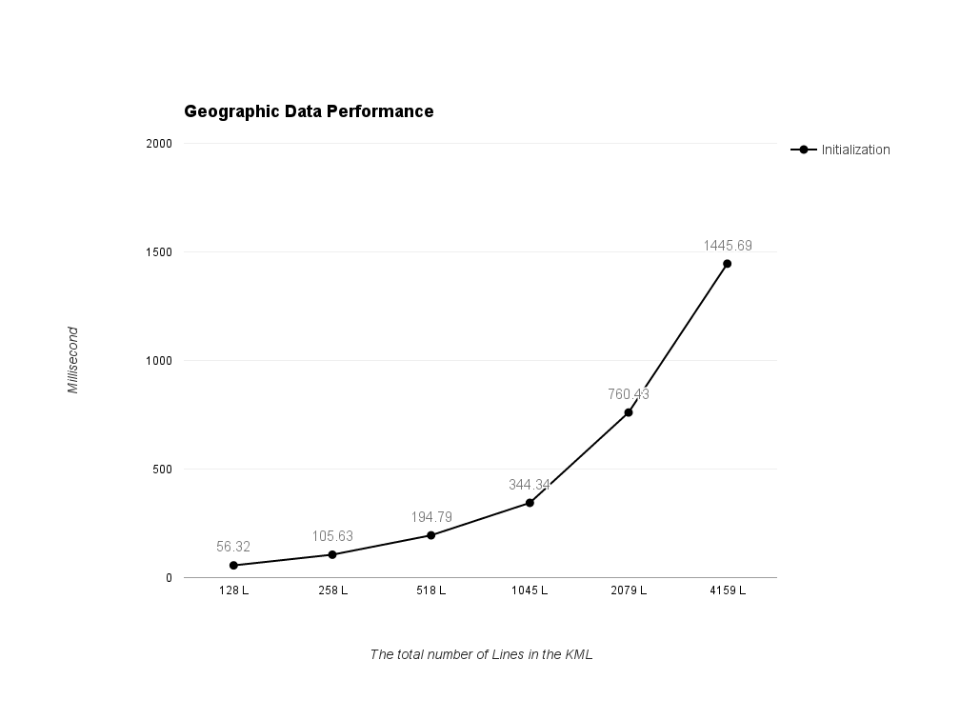
\includegraphics[width=\textwidth, keepaspectratio]{Figures/geographic-data-performance.png}
	\decoRule
\end{figure}

Although, the number could be large, but it is not executed in the UI thread. Additionally, the Earth does not require re-creation when user try to load another scene. Therefore it is not a performance problem.

%****************************************************************
\section{Runtime}

%****************************************************************
Tasks that require continually repeated during the render loop is the factors influencing the runtime performance. They are ray-model intersection detection, update and draw models \ref{fig:cyclic-task}. In this section, I present the tasks that closely related to performance and the memory leak analysis during the loop.
 
\begin{figure}[H]
	\caption{Cyclic Task}
	\label{fig:cyclic-task}
	\centering
	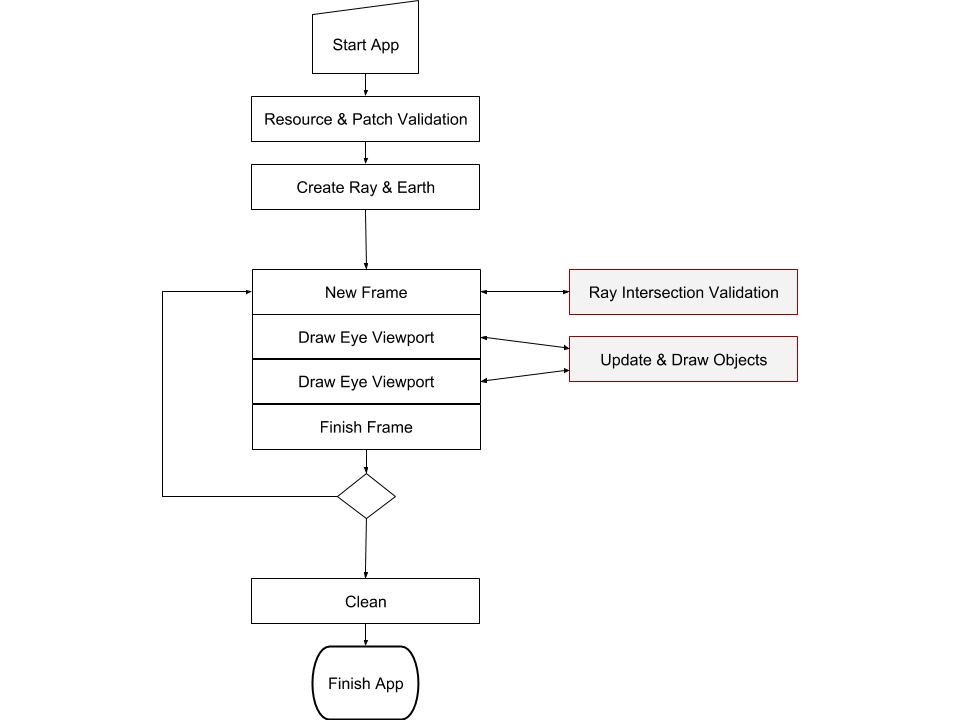
\includegraphics[width=\textwidth, keepaspectratio]{Figures/cyclic-task.png}
	\decoRule
\end{figure}


%****************************************************************
\subsection{Memory Leak}

%****************************************************************
I am using Memory Monitor to evaluate memory leak. As the application allocates and free memory, we will see the allocative amount fluctuate in the graph at the same time. Any time the allocated memory drops by a significant amount, that is a signal that GC event has occurred (see \ref{fig:memory-monitor}). These GC events are not generally a noticeable performance problem. However, lots of them occurring over and over and over again in a short period of time can lead to performance issues. Additionally, it more or less created memory leaks, which are objects which the application is no longer using, but the garbage collector fails to recognize them as unused.

\begin{figure}[H]
	\caption[Memory Monitor]{Memory Monitor \cite{google.memory-monitor.2015}}
	\label{fig:memory-monitor}
	\centering
	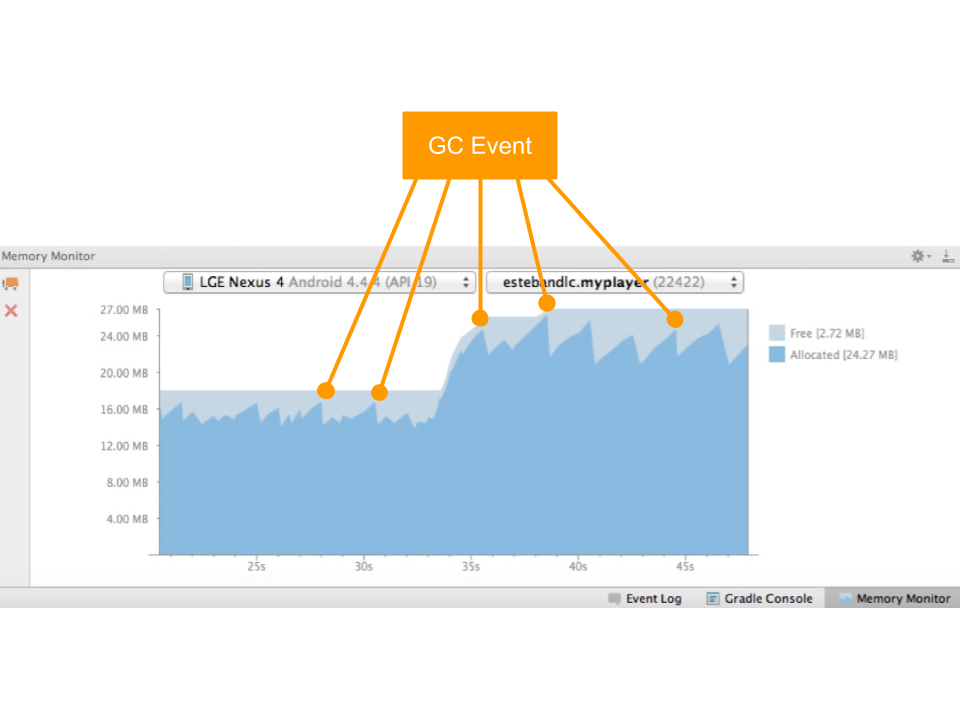
\includegraphics[width=\textwidth, keepaspectratio]{Figures/memory-monitor.png}
	\decoRule
\end{figure}

In a world where the application is not doing much of anything, there will be a flat memory allocation graph. This is an ideal scenario from a performance perspective. The more time is spending doing GC, the less time for the application to do other stuff. Fortunately, with a careful in dealing with objects, I got a quite flat runtime memory allocation \ref{fig:memory-performance}.

\begin{figure}[H]
	\caption{Memory Performance}
	\label{fig:memory-performance}
	\centering
	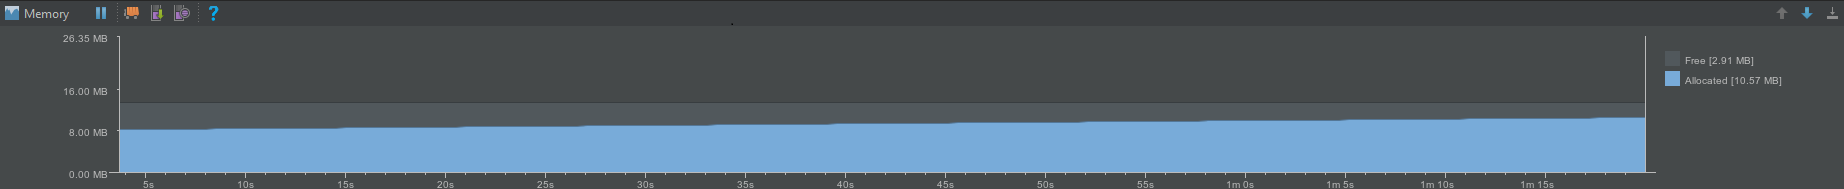
\includegraphics[width=\textwidth, keepaspectratio]{Figures/memory-performance.png}
	\decoRule
\end{figure}

%****************************************************************
\subsection{Placemarks Intersection}
\label{section:placemarks-intersection}

%****************************************************************
There was a significant performance improvement in detecting ray-placemark intersection per frame. In order to avoid doing intersection test on all \code{Placemark} per frame, I implemented Octree space partition to ignore unnecessary detections (see Chart \ref{fig:placemarks-intersection-performance}).

\begin{figure}[H]
	\caption{Placemarks Intersection Performance}
	\label{fig:placemarks-intersection-performance}
	\centering
	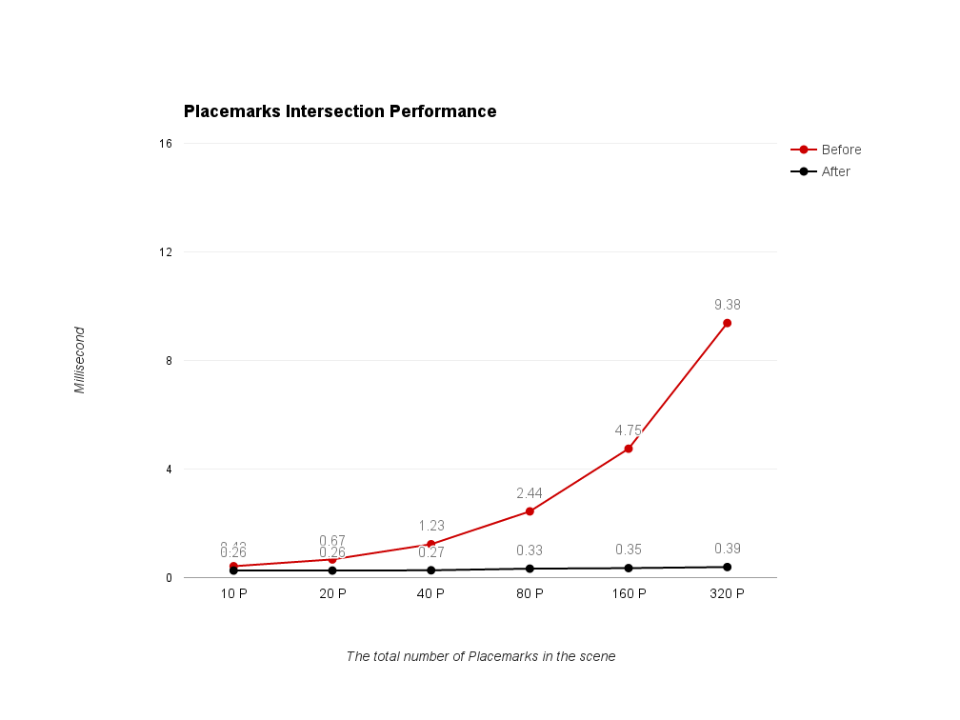
\includegraphics[width=\textwidth, keepaspectratio]{Figures/placemarks-intersection-performance.png}
	\decoRule
\end{figure}

After the optimization, the number is negligible even for $1000$ \code{Placemark} ( less than 2ms).

%****************************************************************
\subsection{Placemarks Update}
\label{section:placemarks-update}

%****************************************************************

There was a incredible performance optimization for ray-placemark update process \ref{fig:placemarks-update-performance}. 

\begin{figure}[H]
	\caption{Placemarks Update Performance}
	\label{fig:placemarks-update-performance}
	\centering
	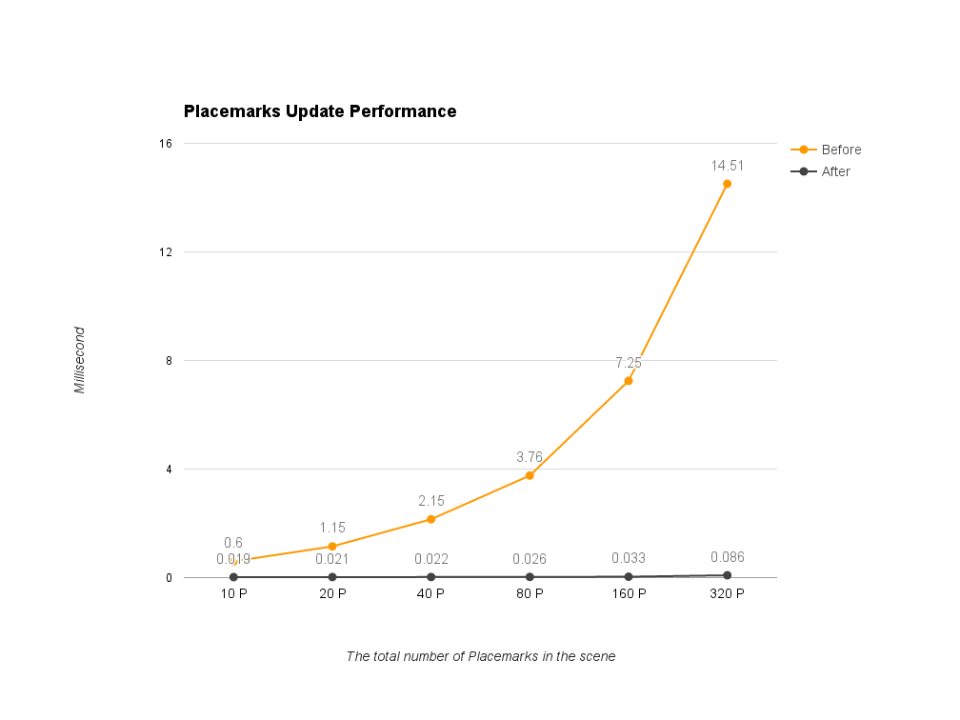
\includegraphics[width=\textwidth, keepaspectratio]{Figures/placemarks-update-performance.png}
	\decoRule
\end{figure}

There are mainly $6$ type of calculations (see Table \ref{tab:opengl-compute-scope}):

\begin{table}[H]
	\caption{OpenGL compute scope}
	\label{tab:opengl-compute-scope}
	\centering
	\begin{tabular}{l l l l}
		\toprule
		\tabhead{What} & \tabhead{How} & \tabhead{Scope}\\
		\midrule
		Model Matrix & translationM * scaleM * rotationM * identityM(1) & Object specific\\
		Camera Matrix & lookAt(positionV, lookAtV, upV) & Worldwide\\
		View Matrix & eye.viewM * cameraM & Eye specific\\
		Perspective Matrix & eye.perspective(zNear, zFar) & Eye specific\\
		ModelView Matrix & viewM * modelM & Object specific\\
		Projection Matrix & perspectiveM * modelViewM & Object specific\\
		Vertex' & projectionM * vertex & Vertex specific\\
		\bottomrule
	\end{tabular}
\end{table}

Before the optimization, based on the \code{viewM} and \code{perspectiveM} from each eye, computing the \code{modelM}, \code{modelViewM} and \code{projectionM} in CPU for each object per frame. Then pass the \code{modelViewM} and \code{projectionM} to GPU for further calculation, such as lighting and position (\code{Vertex'}). It creates huge performance problem, due to a large amount of computation can be omitted. There is no need to re-calculate an object's \code{modelM} per frame if the object has the same position, scale, and rotation. It is the same for \code{modelViewM} and \code{projectionM}. Therefore, after the optimization, application only re-calculate the \code{modelM} for objects which needed, and all objects pass \code{viewM} and \code{perspectiveM} to GPU for the rest of calculation. Although it increases the workload in GPU as well as duplicated calculation, it has improved performance for the application. Dealing with the duplicated calculation in GPU caused by the optimization has been postponed to future work, because it related to optimization of drawing massive \code{Placemark} which has been postponed as well (see the next Section \ref{section:placemarks-draw}).

\begin{table}[H]
	\caption{OpenGL compute optimization}
	\label{tab:opengl-compute-optimization}
	\centering
	\begin{tabular}{l l l l}
		\toprule
		\tabhead{What} & \tabhead{Before} & \tabhead{After}\\
		\midrule
		Model Matrix & Each object (CPU) & Objects are needed (CPU)\\
		Camera Matrix & When moving (CPU) &  When moving (CPU)\\
		View Matrix & Each eye (CPU) & Each eye (CPU)\\
		Perspective Matrix & Each eye (CPU) & Each eye (CPU)\\
		ModelView Matrix & Each object (CPU) & Each Vertex (GPU)\\
		Projection Matrix & Each object (CPU) & Each Vertex (GPU)\\
		Vertex' & Each Vertex (GPU) & Each Vertex (GPU)\\
		\bottomrule
	\end{tabular}
\end{table}


%****************************************************************
\subsection{Placemarks Draw}
\label{section:placemarks-draw}

%****************************************************************
The performance of draw all \code{Placemark} has not been adequate, due to the number of times calling \code{glDrawElements} API, which is an expensive call and it is called during each \code{Placemark} draw process. Anytime the frame takes more than $16$ms barrier, and the user will notice it. Because the two eye's viewports are both need to be updated and re-draw, therefore the update and draw process only has $8$ms in total to do what needs to be done. Although the performance of ray-object intersection and \code{Placemark} update are satisfied, but the performance issues in draw process are significant. The $0.048$ms average time-consuming and $0.046$ms stand deviation indicate that it not only has an unstable value but also it could reach $8$ms by just call the API $170$ times (See Chart \ref{fig:glDrawElements-performance}).

\begin{figure}[H]
	\caption{glDrawElements Performance}
	\label{fig:glDrawElements-performance}
	\centering
	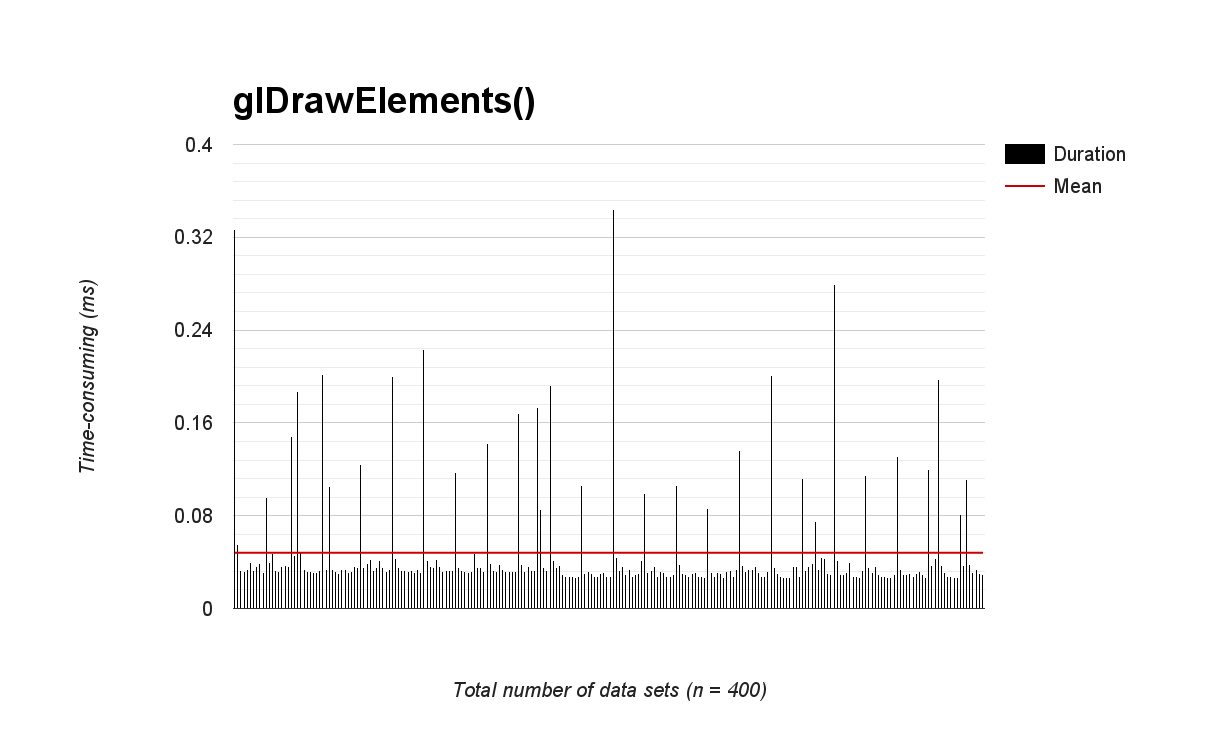
\includegraphics[width=\textwidth, keepaspectratio]{Figures/glDrawElements-performance.png}
	\decoRule
\end{figure}

The solution is straightforward using one \code{glDrawElements} call for all \code{Placemark}. Unfortunately, it has not been optimized yet due to a limited time. In general, using interleaved attributes will do the trick.

%****************************************************************
